%%%%%%%%%%%%%%%%%%%%%%% file template.tex %%%%%%%%%%%%%%%%%%%%%%%%%
%
% This is a template file for The European Physical Journal PLUS
%
% Copy it to a new file with a new name and use it as the basis
% for your article
%
%%%%%%%%%%%%%%%%%%%%%%%% Springer-Verlag / Societa` Italiana di Fisica  %%%%%%%%%%%%%%%%%%%%%%%%%
%
\begin{filecontents}{leer.eps}
\begin{document}
!PS-Adobe-2.0 EPSF-2.0
%%CreationDate: Mon Jul 13 16:51:17 1992
%%DocumentFonts: (atend)
%%Pages: 0 1
%%BoundingBox: 72 31 601 342
%%EndComments

gsave
72 31 moveto
72 342 lineto
601 342 lineto
601 31 lineto
72 31 lineto
showpage
grestore
%%Trailer
%%DocumentFonts: Helvetica
\end{filecontents}
%
\documentclass[epj]{svjour}
% Remove option referee for final version
%
% Remove any % below to load the required packages
%\usepackage{latexsym}
\usepackage{mathtools} % Loads amsmath
\usepackage{graphics}
\usepackage{amsmath}
\usepackage{amssymb}
\usepackage{latexsym}
\usepackage{amsfonts}
\usepackage{authblk}
\usepackage{xfrac}
\usepackage{graphicx}
%\usepackage[colorlinks=true,linkcolor=black, citecolor=blue, urlcolor=blue]{hyperref} % for hyperrefs
%\usepackage{cleveref}
%\usepackage[authoryear]{natbib}
\usepackage{gensymb}  % provides macro \degree which works in text and math
\usepackage{color}
%\usepackage{enumitem} 
\usepackage{bm}
\usepackage{multirow}
\usepackage{cite}
\usepackage{tikz}
%\usetikzlibrary{arrows}
\usetikzlibrary{arrows, arrows.meta}

% for quotes
\usepackage [english]{babel}
\usepackage [autostyle, english = american]{csquotes}
\MakeOuterQuote{"}

% etc
%

\newcommand{\eq}[1]{Eq.~(\ref{#1})}
\newcommand{\eqnolabel}[1]{(\ref{#1})}
\newcommand{\eqs}[1]{Eqs.~(\ref{#1})}
\newcommand{\eqsthru}[2]{Eqs.~(\ref{#1})--(\ref{#2})}
\newcommand{\eqsand}[2]{Eqs.~(\ref{#1}) and (\ref{#2})}
\newcommand{\tbl}[1]{Table~\ref{#1}}
\newcommand{\tblnolabel}[1]{\ref{#1}}
\newcommand{\tbls}[1]{Tables~\ref{#1}}
\newcommand{\tblsthru}[2]{Tables~\ref{#1}--\ref{#2}}
\newcommand{\tblsand}[2]{Tables~\ref{#1} and \ref{#2}}
\newcommand{\fig}[1]{Fig.~\ref{#1}}
\newcommand{\fignolabel}[1]{\ref{#1}}
\newcommand{\figs}[1]{Figs.~\ref{#1}}
\newcommand{\figsthru}[2]{Figs.~\ref{#1}--\ref{#2}}
\newcommand{\figsand}[2]{Figs.~\ref{#1} and \ref{#2}}
\newcommand{\sxn}[1]{Section~\ref{#1}}

\newcommand{\revised}[1]{{\color{red}{#1}}}
\newcommand{\tsup}[1]{\textsuperscript{#1}}
\newcommand{\tsub}[1]{\textsubscript{#1}}

\newcommand{\erez}[1]{{\color{blue}{\textsuperscript{EREZ:}#1}}}
\newcommand{\roy}[1]{{\color{blue}{\textsuperscript{ROY:}#1}}}

\newcommand{\keff}{{\ensuremath{k_{\textrm{\scriptsize{eff}}}}}}
\newcommand{\beff}{\ensuremath{\beta_{\textrm{eff}}}}
\newcommand{\rr}{\ensuremath{\bm{r}}}
\newcommand{\OO}{\ensuremath{\hat{\bm{\Omega}}}}
\newcommand{\bnabla}{\ensuremath{\bm{\nabla}}}
\newcommand{\rE}{\ensuremath{(\rr,E)}}

\newcommand{\ftr}{\ensuremath{\phi_{\textrm{\scriptsize{tr}}}}}
\newcommand{\jtr}{\ensuremath{\bm{J}_{\textrm{\scriptsize{tr}}}}}
\newcommand{\jtrr}{\ensuremath{J_{\textrm{\scriptsize{tr}}}}}
\newcommand{\mcL}{\mathcal{L}}
\newcommand{\pl}[1]{\ensuremath{P_l(#1)}}
\newcommand{\dx}{\ensuremath{\Delta x}}


% For merging cells 
\usepackage{array}
\usepackage{booktabs}
\setlength{\heavyrulewidth}{1.5pt}
\setlength{\abovetopsep}{4pt}

% ---------------------------------------------------
\begin{document}


\begin{figure}[htbp!] 
	\centering
	For $x>x'$.
	\begin{tikzpicture}
	\tikzstyle{every node}=[font=\footnotesize]
	\draw[thick] (0,0) -- (7.5,0);
	\draw[thick,->] (8.5,0) -- (16,0) node[anchor=west] {$x$};
	
	
	\node[anchor=south] at (1cm,1pt) {$x_{j-1}$};
	\node[anchor=north] at (1cm,-1pt) {$\sigma_{g,j-1}$};
	
	\draw ( 3 cm,2pt) -- ( 3 cm,-2pt) node[anchor=north] {$x_{j-1/2}$};
	\node[anchor=south] at (5cm,1pt) {$x_j$};
	\node[anchor=north] at (5cm,-1pt) {$\sigma_{g,j}$};
	\draw ( 7 cm,2pt) -- ( 7 cm,-2pt) node[anchor=north] {$x_{j+1/2}$};
	
	\node[anchor=south] at (8cm,-5pt) {$\ldots$};
	
	%\node[anchor=south] at (9cm,1pt) {$x_{j-1}$};
	
	\draw ( 10 cm,2pt) -- ( 10 cm,-2pt) node[anchor=north] {$x_{i-1/2}$};
	\node[anchor=south] at (12cm,1pt) {$x_{i}$};
	\node[anchor=north] at (12cm,-1pt) {$\sigma_{g,i}$};
	%\node[anchor=south] at (16.5cm,1pt) {$x_{j+1/2}$};
	\draw ( 14 cm,2pt) -- ( 14 cm,-2pt) node[anchor=north] {$x_{i+1/2}$};
	
	\node[anchor=south] at (4cm,2pt) {$x'$};
	
	% ------------------- Vertical dashed lines ------------------- %
	\draw [dashed] ( 7 cm, -0.5cm) -- ( 7 cm,-1.2cm);
	\draw [dashed] ( 14 cm, -0.5cm) -- ( 14 cm,-2.1cm);
	\draw [dashed] ( 4 cm, 0.1cm) -- ( 4 cm,-2.1cm);	
	
	% ------------------- Horizontal arrows + text ------------------- %
	\draw[>=triangle 45, <->] (7cm,-1.2cm) -- (14cm,-1.2cm);
	\node[anchor=south] at (10.5cm,-1.2cm) {$\Xi_{i,j}^g$};
	
	\draw[>=triangle 45, <->] (4cm,-2.1cm) -- (14cm,-2.1cm);
	\node[anchor=south] at (9cm,-2.1cm) {$\Xi_{i,j}^g + \sigma_{g,j}\left(x_{j+1/2} - x'\right)$};
	
	\end{tikzpicture}
\bigbreak
\bigbreak
For $x<x'$.
\begin{tikzpicture}
\tikzstyle{every node}=[font=\footnotesize]
\draw[thick] (0,0) -- (7.5,0);
\draw[thick,->] (8.5,0) -- (16,0) node[anchor=west] {$x$};

\node[anchor=south] at (1cm,1pt) {$x_{i-1}$};
\node[anchor=north] at (1cm,-1pt) {$\sigma_{g,i-1}$};

\draw ( 3 cm,2pt) -- ( 3 cm,-2pt) node[anchor=north] {$x_{i-1/2}$};
\node[anchor=south] at (5cm,1pt) {$x_i$};
\node[anchor=north] at (5cm,-1pt) {$\sigma_{g,i}$};
\draw ( 7 cm,2pt) -- ( 7 cm,-2pt) node[anchor=north] {$x_{i+1/2}$};

\node[anchor=south] at (8cm,-5pt) {$\ldots$};

%\node[anchor=south] at (9cm,1pt) {$x_{j-1}$};

\draw ( 10 cm,2pt) -- ( 10 cm,-2pt) node[anchor=north] {$x_{j-1/2}$};
\node[anchor=south] at (12cm,1pt) {$x_{j}$};
\node[anchor=north] at (12cm,-1pt) {$\sigma_{g,j}$};
%\node[anchor=south] at (16.5cm,1pt) {$x_{j+1/2}$};
\draw ( 14 cm,2pt) -- ( 14 cm,-2pt) node[anchor=north] {$x_{j+1/2}$};

\node[anchor=south] at (13cm,2pt) {$x'$};

% ------------------- Vertical dashed lines ------------------- %
\draw [dashed] ( 7 cm, -0.5cm) -- ( 7 cm,-2.1cm);
\draw [dashed] ( 10 cm, -0.5cm) -- ( 10 cm,-1.2cm);
\draw [dashed] ( 13 cm, 0.1cm) -- ( 13 cm,-2.1cm);	

% ------------------- Horizontal arrows + text ------------------- %
\draw[>=triangle 45, <->] (7cm,-1.2cm) -- (10cm,-1.2cm);
\node[anchor=south] at (8.5cm,-1.2cm) {$\Xi_{i,j}^g$};

\draw[>=triangle 45, <->] (7cm,-2.1cm) -- (13cm,-2.1cm);
\node[anchor=south] at (10cm,-2.1cm) {$\Xi_{i,j}^g + \sigma_{g,j}\left(x'-x_{j-1/2}\right)$};
\end{tikzpicture}
\bigbreak
\caption{Notation for numerical evaluation of integral interface currents.}
\label{fig:Xi}
\end{figure}


% --------------------------------- Tables --------------------------------- %

\begin{table}[!htbp]
\label{tab:XS}
\centering
\begin{tabular}{cccccc}
\toprule
Group g &  $\Sigma_{t,g}$ & \multicolumn{2}{c}{$\Sigma_{s,0,g\leftarrow g'}$} & $\chi_g$ & $\nu\Sigma_{f,g}$ \\ 
\midrule
1 & $5.3115\cdot 10^{-1}$ & $5.04664\cdot 10^{-1}$ & $2.03884\cdot 10^{-3}$ & 1 & $7.15848\cdot 10^{-3}$ \\
\midrule
2 & $1.30058\cdot 10^{+0}$& $1.62955\cdot 10^{-2}$ & $1.19134\cdot 10^{+0}$	& 0 & $1.41284\cdot 10^{-1}$ \\
\bottomrule
\end{tabular}
\end{table}




\begin{table}[!htbp]
\label{tab:dx_drho}
\centering
\begin{tabular}{lccc}
\toprule
$dx(I) [cm]$  &  $k_{\text{ref}}$ & $k_{\text{RM}}$ & $\Delta\rho [pcm]$\\ 
\midrule
0.43(50)     & 0.744307 & 0.740552  & -681\\
\midrule
0.215(100)    & 0.744391 & 0.743447 & -171\\
\midrule
0.1075(200)   & 0.744412 & 0.744212 & -36\\
\midrule
0.071667(300) & 0.744416 & 0.744356 & -11\\
\midrule
0.05375(400)  & 0.744417 & 0.744407 & -2\\
\bottomrule
\end{tabular}
\end{table}


% -----------------------------------------------------------------------------

\begin{figure}[htbp!] 
	\centering
	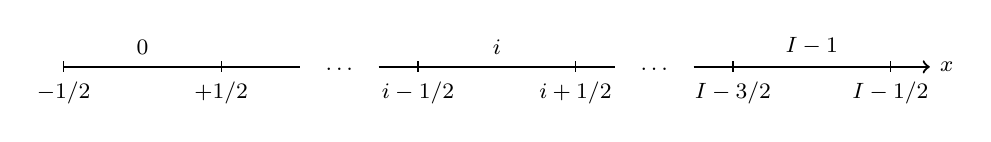
\begin{tikzpicture}
	\tikzstyle{every node}=[font=\footnotesize]
	\draw[thick] (0,0) -- (3,0);
	\node[anchor=south] at (3.5cm,-5pt) {$\ldots$};
	\draw[thick] (4,0) -- (7,0);
	\node[anchor=south] at (7.5cm,-5pt) {$\ldots$};
	\draw[thick,->] (8,0) -- (11,0) node[anchor=west] {$x$};
	
	\draw ( 0 cm,2pt) -- ( 0 cm,-2pt) node[anchor=north] {$-1/2$};
	\node[anchor=south] at (1cm,1pt) {0};
	\draw ( 2 cm,2pt) -- ( 2 cm,-2pt) node[anchor=north] {$+1/2$};

	\draw ( 4.5 cm,2pt) -- ( 4.5 cm,-2pt) node[anchor=north] {$i-1/2$};
	\node[anchor=south] at (5.5cm,1pt) {$i$};
	\draw ( 6.5 cm,2pt) -- ( 6.5 cm,-2pt) node[anchor=north] {$i+1/2$};

	\draw ( 8.5 cm,2pt) -- ( 8.5 cm,-2pt) node[anchor=north] {$I-3/2$};
	\node[anchor=south] at (9.5cm,1pt) {$I-1$};
	\draw ( 10.5 cm,2pt) -- ( 10.5 cm,-2pt) node[anchor=north] {$I-1/2$};
	\end{tikzpicture}
	\end{figure}
\end{document}



